\documentclass[10pt, pdf, hyperref={unicode}]{beamer}
\usetheme{metropolis} 

\usepackage{polyglossia}
\setdefaultlanguage[spelling=modern]{russian}

\usepackage{caption}
\captionsetup[figure]{labelformat=empty, font=scriptsize}

\usepackage{bibentry}
\nobibliography*

%\setbeamerfont{bibliography item}{size=\tiny}
%\setbeamerfont{bibliography entry author}{size=\tiny}
%\setbeamerfont{bibliography entry title}{size=\tiny}
%\setbeamerfont{bibliography entry location}{size=\tiny}
%\setbeamerfont{bibliography entry note}{size=\tiny}

\title{Оптический отклик Ми-резонансных наночастиц, связанных с диэлектрическими волноводами}
\date{}
\author{Нестеров~К.\,Е.}
\institute{
	МОСКОВСКИЙ ГОСУДАРСТВЕННЫЙ УНИВЕРСИТЕТ имени М.В.ЛОМОНОСОВА \\
	ФИЗИЧЕСКИЙ ФАКУЛЬТЕТ МГУ \\
	Кафедра квантовой электроники
}

\begin{document}
  	\maketitle
  
  	\begin{frame}{Оптические метаматериалы}
    \begin{minipage}[b]{.5\textwidth}
    	Неметаллические
    	\begin{figure}
    		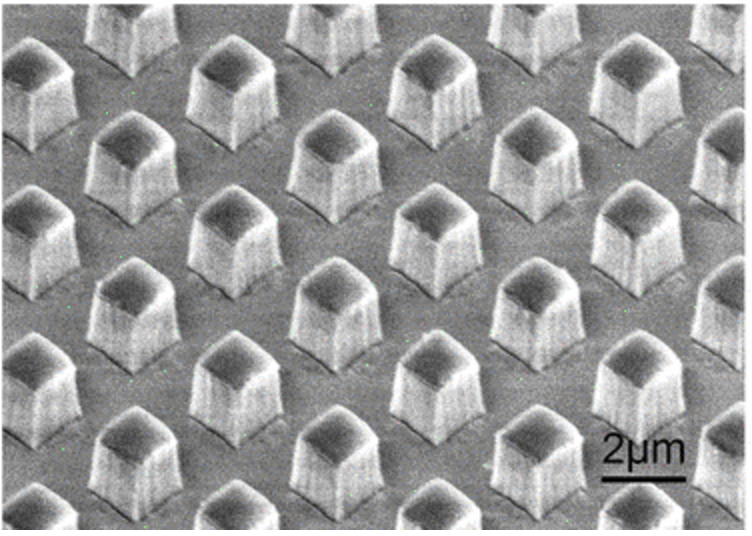
\includegraphics[width=\textwidth]{img/Ginn}
    		\caption{\bibentry{Ginn2012}}
    	\end{figure}
    \end{minipage}
\end{frame}
  
  	\bibliographystyle{presentation}
	\bibliography{literature-abbrv}
\end{document}